{\Huge \textbf{\textcolor{Maroon}{ASP}}:} 
\begin{figure}[ht!]
    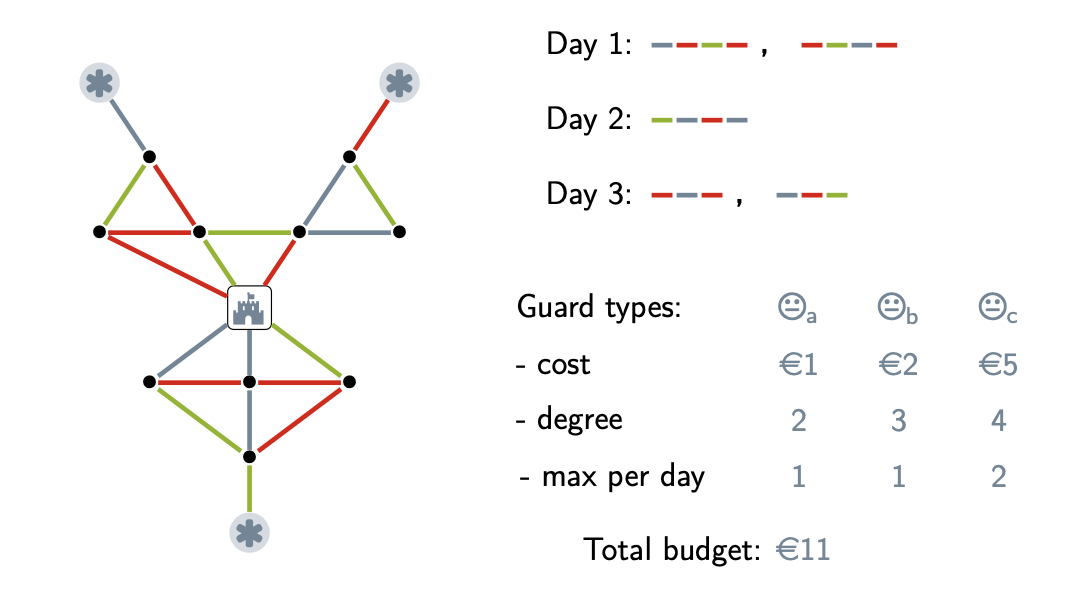
\includegraphics[scale=0.65]{figures/towerdef.png}
\end{figure}

\textbf{Details}: 
\begin{itemize}
    \setlength\itemsep{0em}
    \item You have to protect your tower for as many days as possible
    \item Each day, several waves of attackers come from the nodes
    \begin{itemize}
        \setlength\itemsep{0em}
        \item You don’t know which node they come from—you have to consider any strategy that they might use 
        \item Different waves can come from different nodes (or from the same)
    \end{itemize}
    \item The waves can only pass along edges with a certain sequence of \textcolor{Blue}{c}\textcolor{Red}{o}\textcolor{Green}{l}\textcolor{Blue}{o}\textcolor{Red}{r}\textcolor{Green}{s}
    \item Each day, you can place some guards on some nodes (not on tower, not on node)
    \begin{itemize}
        \setlength\itemsep{0em}
        \item Guards will stop all attackers on that node (on that day)
        \item There are different guard types, each with (i) their own cost, (ii) restrictions on the degree of nodes that they can be placed on, and (iii) maximum number of guards of that type that can be placed on any given day
    \end{itemize}
    \item Given some budget, what is the maximum number of days that you can survive?
\end{itemize}

\newpage

{\Huge \textbf{\textcolor{MidnightBlue}{Encode input}}}  \\
\\

{\Large \textbf{\textcolor{Maroon}{Representing the graph}}:} 

\begin{lstlisting}
$\text{\textcolor{PineGreen}{\% Nodes and colored edges}}$
node(1..14).
edge(1,3,blue).
edge(3,6,red).
edge(3,5,green).
edge(5,6,red).
edge(6,7,green).
edge(7,8,blue).
edge(2,4,red).
edge(4,7,blue).
edge(4,8,green).
edge(5,9,red).
edge(6,9,green).
edge(7,9,red).
edge(9,10,blue).
edge(9,11,blue).
edge(9,12,green).
edge(10,11,red).
edge(11,12,red).
edge(10,13,green).
edge(11,13,blue).
edge(12,13,red).
edge(13,14,green).

$\text{\textcolor{PineGreen}{\% Edges are also reversed}}$
edge(X,Y,C) :- edge(Y,X,C).

$\text{\textcolor{PineGreen}{\% Tower}}$
tower(9).

$\text{\textcolor{PineGreen}{\% Spawn points}}$
spawn(1).
spawn(2).
spawn(14).
\end{lstlisting}

\newpage

{\Large \textbf{\textcolor{Maroon}{Representing the waves}}:} 
\begin{lstlisting}
$\text{\textcolor{PineGreen}{\% Waves -- wave\_on\_day(W,D) indicates that wave W happens on day D}}$
$\text{\textcolor{PineGreen}{\% wave(W,I,C) indicates that the I'th step in wave W has color C}}$
wave_on_day(1,1).
wave(1,1,blue).
wave(1,2,red).
wave(1,3,green).
wave(1,4,red).
wave_on_day(2,1).
wave(2,1,red).
wave(2,2,green).
wave(2,3,blue).
wave(2,4,red).
wave_on_day(3,2).
wave(3,1,green).
wave(3,2,blue).
wave(3,3,red).
wave(3,4,blue).
wave_on_day(4,3).
wave(4,1,red).
wave(4,2,blue).
wave(4,3,red).
wave_on_day(5,3).
wave(5,1,blue).
wave(5,2,red).
wave(5,3,green).
% wave(W) :- wave_on_day(W,_).
\end{lstlisting}

\vspace{0.40cm}

{\Large \textbf{\textcolor{Maroon}{Representing the guard types and budget}}:} 
\begin{lstlisting}
$\text{\textcolor{PineGreen}{\% Guard types}}$
guard_type(a;b;c).
guard_type_degree(a,2).
guard_type_degree(b,3).
guard_type_degree(c,4).
guard_type_cost(a,1).
guard_type_cost(b,2).
guard_type_cost(c,5).
guard_type_limit_per_day(a,1).
guard_type_limit_per_day(b,1).
guard_type_limit_per_day(c,2).

$\text{\textcolor{PineGreen}{\% Budget}}$
budget(12).
\end{lstlisting}

\newpage 

{\Huge \textbf{\textcolor{MidnightBlue}{Encode candidate solutions}}}  \\
\\

{\Large \textbf{\textcolor{Maroon}{Choosing a number of days to survive}}:} 
\begin{lstlisting}
$\text{\textcolor{PineGreen}{\% Choose a sequence of days day(1), ..., day(j) to survive}}$
max_day(D) :- D = #max { E : wave_on_day(_,E) }.
possible_day(D) :- max_day(D).
possible_day(D-1) :- possible_day(D), D > 1.
{ day(D) : possible_day(D) }.
:- day(D), possible_day(D-1), not day(D-1). $\text{\textcolor{PineGreen}{\% symmetry breaking}}$ 
    $\text{\textcolor{PineGreen}{\% days that we play must be subsequent: 1,2,...}}$
\end{lstlisting}

\vspace{0.40cm}

{\Large \textbf{\textcolor{Maroon}{Choosing a basic strategy}}:} 
\begin{lstlisting}
$\text{\textcolor{PineGreen}{\% Choose a strategy for placing guard on nodes on different days}}$
$\text{\textcolor{PineGreen}{\% place(D,G,N) indicates that on day D, a guard of type G is placed on node N}}$
{ place(D,G,N) : day(D), guard_type(G), node(N) }.

$\text{\textcolor{PineGreen}{\% Guards cannot be placed on spawn points or on the tower}}$
:- place(D,G,N), spawn(N).
:- place(D,G,N), tower(N).
\end{lstlisting}

\vspace{1cm}

{\Huge \textbf{\textcolor{MidnightBlue}{Encode solution properties}}}  \\
\\
{\Large \textbf{\textcolor{Maroon}{Respect budget, check guard restrictions and compute degree of nodes}}:}
\begin{lstlisting}
$\text{\textcolor{PineGreen}{\% Compute the degree of nodes}}$
degree(N,D) :- node(N), D = #count { M : edge(N,M,C) }.

$\text{\textcolor{PineGreen}{\% Ensure that guard types are only placed on nodes with the allowed degree}}$
:- place(D,G,N), day(D), guard_type(G),
   guard_type_degree(G,E), not degree(N,E).

$\text{\textcolor{PineGreen}{\% Ensure that on each day, the limits on the different guard types are respected}}$
guard_type_used_per_day(G,D,M) :- 
    guard_type(G), day(D),
    M = #count { N : place(D,G,N) }.
   
:- guard_type_used_per_day(G,D,M), 
    guard_type(G), day(D),
    guard_type_limit_per_day(G,L), M > L.
\end{lstlisting}

\newpage

{\Large \textbf{\textcolor{Maroon}{Checking that the tower remains safe}}:}
\begin{lstlisting}
$\text{\textcolor{PineGreen}{\% Derive what nodes the different waves can reach}}$
$\text{\textcolor{PineGreen}{\% reachable(W,D,N,I) indicates that wave W (up to index I) can reach node N on day D}}$
reachable(W,D,N,0) :- wave_on_day(W,D), spawn(N).
reachable(W,D,N,I) :- wave_on_day(W,D), I > 0,
    reachable(W,D,M,I-1), edge(M,N,C), wave(W,I,C),
    not place(D,G,N) : guard_type(G).

$\text{\textcolor{PineGreen}{\% Ensure that the tower is never reached (after any part of a wave)}}$
:- day(D), tower(N), reachable(_,D,N,_).
\end{lstlisting}

\vspace{1cm}

{\Huge \textbf{\textcolor{MidnightBlue}{Optimization}}} \\
\\
{\Large \textbf{\textcolor{Maroon}{Maximizing the number of survived days}}:}
\begin{lstlisting}
$\text{\textcolor{PineGreen}{\% Maximize the number of days survived}}$
#maximize { 1,day(D) : day(D) }.
\end{lstlisting}

\vspace{0.5cm}

{\Large \textbf{\textcolor{Maroon}{Show}}:}
\begin{lstlisting}
$\text{\textcolor{PineGreen}{\% Show only the strategy and how which days survived}}$
#show day/1.
#show place/3.
\end{lstlisting}

\newpage

{\Huge \textbf{\textcolor{Maroon}{Now using propositional logic}}:} \\
\\
\\
We will construct a \textbf{CNF formula $\varphi_k$} that:
\begin{itemize}
    \setlength\itemsep{0em}
    \item is \textcolor{NavyBlue}{is statisfiable} if and only if there is a strategy to survive the first $k$ days,
    \item has satisfying assignments that correspond to strategies to survive the first $k$ days.
\end{itemize}

\vspace{0.5cm}

We introduce propositional variables $p_{d\; ,g\; ,n}$ for each day $d \in \{1, \ldots, k\}$, each guard type $g$ and each node $n$.
\begin{itemize}
\setlength\itemsep{0em}
    \item The truth assignment to these variables will represent the strategy: \\
    \textcolor{NavyBlue}{$p_{d\; ,g\; ,n}$ represents whether on day $d$ we place a guard of type $g$ on node $n$.}
    \item All other variables that we introduce will only be auxiliary variables that we use to express the various constraints.
\end{itemize}

For each tower or node $n$, and each day $d \in \{1, \ldots, k\}$ and guard type $g$, we add the clause:
$$ (\neg p_{d\; ,g\; ,n}) $$

\vspace{1cm}

{\Large \textbf{\textcolor{Maroon}{Expressing the degree restrictions}}:} 
\begin{itemize}
    \item Let $\mathbf{d}(n)$ be the degree of a node, and let $\mathbf{d}(g)$ be the degree of nodes that guards of type $g$ may be placed on.
    \item For each node $n$, for each guard type $g$ such that $\boldsymbol{d}(n) \neq \boldsymbol{d}(g)$, and for each day $d \in\{1, \ldots, k\}$, we add the clause:
    $$
    \left(\neg p_{d, g, n}\right)
    $$ 
\end{itemize}

\vspace{1cm}

{\Large \textbf{\textcolor{Maroon}{First auxiliary variables}}:} \\
We add auxiliary variables $q_{d\;, n}$ to represent whether on day $d$ node $n$ is guarded. To \textbf{enforce} this, we add the following clauses:
\begin{align*}
    \left(\neg p_{d, g, n} \vee q_{d, n}\right) &\text{ for each } d, g, n ; \\
    (\neg q_{d, n} \vee \bigvee_{g \in G} p_{d, g, n}) &\text{ for each } d, n;
\end{align*}

\newpage

{\Large \textbf{\textcolor{Maroon}{Expressing reachability}}:} \\
We add variables $r_{d, w, n, i}$ to represent whether wave $w$ on day $d$ can reach node $n$ after $i$ steps. To \textbf{enforce} this, we add the following clauses: 
\begin{equation*}
\begin{aligned}
&\begin{array}{ll}
\left(r_{d, w, n, 0}\right) & \text { for each } d, w \text { and each} \text { node } n ; \\
\left(\neg r_{d, w, n_{1}, i} \vee q_{d, n_{2}} \vee r_{d, w, n_{2}, i+1}\right) & \text { for each } d, w, i, n_{1}, n_{2} \text { such that there is an } \\
\left(\neg q_{d, n_{2}} \vee \neg r_{d, w, n_{2}, i+1}\right) & \text { edge between } n_{1} \text { and } n_{2} \text { with color } c \text {, where } \\
& \text { the }(i+1) \text {-th 'leg' of } w \text { has color } c \text {; } \\
\left(\bigvee_{n_{2} \in N_{c}} r_{d, w, n_{2}, i} \vee \neg r_{d, w, n_{1}, i+1}\right) & \text { for each } d, w, i, n_{1} \text { where } N_{c} \text { is the set of } \\
\left(\neg q_{d, n_{2}} \vee \neg r_{d, w, n_{2}, i+1}\right) & \text { nodes } n_{2} \text { with an edge of color } c \text { to node } n_{1} \\
& \text { and where the }(i+1) \text {-th 'leg' of } w \text { has } \\
& \text { color } c \text {; }
\end{array}
\end{aligned}
\end{equation*}

Finally, for each tower node $n$, and each $d, w, i$, we add the clause: $$\left(\neg r_{d, w, n, i}\right)$$

\vspace{1cm}

{\Large \textbf{\textcolor{Maroon}{Expressing the budget restrictions}}:} \\
\\
Let's order the variables $p_{d, g, n}$ in some order: $p_{1}, \ldots, p_{u}$.
\begin{itemize}
    \item So $p_{1}, \ldots, p_{u}$ are just different names that we use to refer to the variables $p_{d, g, n}$, for the sake of presentation.
\end{itemize}

We add variables $s_{j, b}$ for each $0 \leq j \leq u$ and each $0 \leq b \leq$ budget to represent whether the assignment of variables $p_{1}, \ldots, p_{j}$ corresponds to spending $b$. \\
\\
To enforce this, we add the following clauses:
$$
\begin{array}{ll}
\left(s_{0,0}\right) &  \\
\left(\neg s_{0, b}\right) & \text { for each } b>0 ;  \\
\left(\neg s_{j-1, b-c} \vee \neg p_{j} \vee s_{j, b}\right) & \text { for each } j>0, \text { where } p_{j} \text { is a variable for guard placement }  \\
\left(s_{j-1, b-c} \vee \neg p_{j} \vee \neg s_{j, b}\right) & \text { with cost } c, \text { and for each } b \geq c ;  \\
\left(\neg p_{j} \vee \neg s_{j, b}\right) & \text { for each } j>0, \text { where } p_{j} \text { is a variable for guard placement }  \\
& \text { with cost } c, \text { and for each } b<c ; \\
\left(\neg s_{j-1, b} \vee p_{j} \vee s_{j, b}\right) & \text { for each } j>0 \text { and for each } b ; \\
\left(s_{j-1, b} \vee p_{j} \vee \neg s_{j, b}\right) & 
\end{array}
$$

\vspace{0.5cm}

Finally, we add the following constraint that expresses that we must stay within the budget:
\begin{align*}
    (&\;\;\;\;\;\; \bigvee \;\;\;\;\;\; s_{u,b}) \\
    &1 \leq b \leq \text { budget }
\end{align*} 

\newpage

{\Large \textbf{\textcolor{Maroon}{Expressing the budget restrictions}}:} \\
\\
To express the constraints that on each individual day, only a limited number of guards of type g may be placed, we would need to do the following:
\begin{itemize}
    \setlength\itemsep{0em}
    \item For each day $d$, and each guard type $g$, we need to add auxiliary variables to express how many guards of type $g$ have been placed on day $d$.
    \item And we need to add clauses that enforce this intended meaning, and that express that these amounts are within the limit, for each $d$ and each $g$.
    \item (The details are similar to the budget restrictions, and we don’t show them here.)
\end{itemize}

\vspace{1cm}

{\Large \textbf{\textcolor{Maroon}{Expressing the budget restrictions}}:} \\
\\
In propositional logic we cannot express optimization statements, so to find the largest number of days that we can survive, we do the following:
\begin{itemize}
    \setlength\itemsep{0em}
    \item Construct all the formulas $\varphi_{1}, \varphi_{2}, \varphi_{3}, \ldots, \varphi_{m}$, where $m$ is the number of days.
    \item If $\varphi_{i}$ is satisfiable, then $\varphi_{i-1}$ is also satisfiable. \\
    If $\varphi_{i}$ is unsatisfiable, then $\varphi_{i+1}$ is also unsatisfiable. \\
    So $\varphi_{1}, \ldots, \varphi_{\ell}$ are satisfiable and $\varphi_{\ell+1}, \ldots, \varphi_{m}$ are unsatisfiable, for some $\ell$.
    \item Use a SAT solver to check which formulas are satisfiable.
    \item The first $\ell$ for which $\varphi_{\ell+1}$ is unsatisfiable is the maximum number of days that you can survive.
    \item To compute a strategy to survive $\ell$ days, look at the truth assignment that satisfies $\varphi_{\ell}$.
\end{itemize}